\subsection{UC3 - Modifica dei Metadati}
\label{sub:uc3}

\begin{figure}[h]
    \centering
    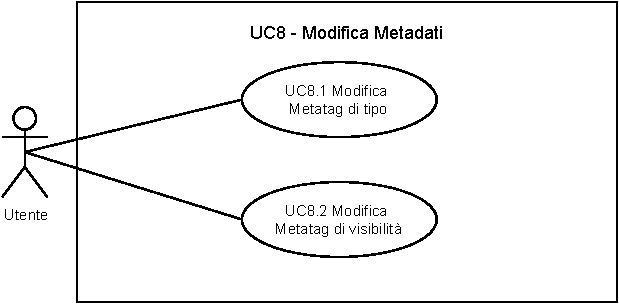
\includegraphics[width=0.7\textwidth]{componenti/casi-duso/diagrammi/UC3.pdf}
    \caption{Diagramma rappresentante UC3}
    \label{fig:UC3}
\end{figure}

%TODO: Modifica immagine
\begin{itemize}
    \item \textbf{Descrizione}: L’utente seleziona una dimensione e modifica i metadati di interesse;
	
    \item \textbf{Attore primario}: Utente;
    
    \item \textbf{Precondizione}:   É stato creato un ambiente valido (\hyperref[sub:uc1]{UC1});
    \item \textbf{Postcondizione}:  Sono stati aggiornati i metadati modificati della dimensione scelta dall'utente e 
    sono state aggiornate eventuali visualizzazioni presenti, in accordo con i metadati aggiornati;

	\item \textbf{Scenario principale}:
        \begin{enumerate}
                \item L'utente seleziona una dimensione da modificare (\hyperref[ssub:uc3.1]{UC3.1});
                \item L'utente modifica il metadato di tipo e/o quello di visibilità della dimensione selezionata 
                (\hyperref[ssub:uc3.2]{UC3.2} e \hyperref[ssub:uc3.3]{UC3.3});
                \item Vengono aggiornati i metadati modificati della dimensione selezionata;
                \item Vengono aggiornate le eventuali visualizzazioni presenti, in accordo con i metadati 
                aggiornati.
        \end{enumerate}

    \item \textbf{Scenari alternativi}:
    \begin{itemize}
        \item L'utente interrompe le modifiche che stava apportando:
        \begin{enumerate}
            \item L'utente seleziona una dimensione da modificare (\hyperref[ssub:uc3.1]{UC3.1});
            \item L'utente deseleziona la dimensione selezionata.
        \end{enumerate}
    \end{itemize}
\end{itemize}

\newpage

\subsubsection{UC3.1 - Scelta della dimensione da modificare}
\label{ssub:uc3.1}

\begin{itemize}
    \item \textbf{Descrizione}: L’utente seleziona una dimensione della quale modificare i metadati;
    \item \textbf{Attore primario}: Utente;

    \item \textbf{Precondizione}:   L'utente ha aperto il menu di modifica dei metadati;
    \item \textbf{Postcondizione}:  Viene selezionata la dimensione del dataset della quale desidera modificare i 
    metadati;

    \item \textbf{Scenario principale}:
    \begin{enumerate}
        \item L'utente seleziona una dimensione tra quelle del dataset corrente.
    \end{enumerate}
\end{itemize}

\subsubsection{UC3.2 - Modifica metadato di tipo}
\label{ssub:uc3.2}

\begin{itemize}
    \item \textbf{Descrizione}: L’utente modifica il metadato di tipo, della dimensione del dataset selezionata, 
    scegliendo il nuovo valore tra le opzioni presentate;
	
    \item \textbf{Attore primario}: Utente;
    
    \item \textbf{Precondizione}:   L'utente ha selezionato una dimensione del dataset della quale desidera modificare 
    i metadati (\hyperref[ssub:uc3.1]{UC3.1});
    \item \textbf{Postcondizione}:  Viene modificato il metadato di tipo della dimensione selezionata;

	\item \textbf{Scenario principale}:
	\begin{enumerate}
        \item L'utente seleziona il metadato di tipo della dimensione precedentemente selezionata;
        \item L'utente seleziona il valore che desidera assegnare al metadato di tipo della dimensione selezionata 
        scegliendo tra i valori proposti.
    \end{enumerate}
    
   
\end{itemize}


\subsubsection{UC3.3 - Modifica metadato di visibilità}
\label{ssub:uc3.3}

\begin{itemize}
    \item \textbf{Descrizione}: L’utente modifica il metadato di visibilità della dimensione del dataset selezionata;
	
    \item \textbf{Attore primario}: Utente;
    
    \item \textbf{Precondizione}:   L'utente ha selezionato una dimensione del dataset della quale desidera modificare 
    i metadati (\hyperref[ssub:uc3.1]{UC3.1});

    \item \textbf{Postcondizione}:  Viene modificato il metadato di visibilità della dimensione selezionata;

    \item \textbf{Scenario principale}: 
    \begin{enumerate}
        \item L'utente seleziona il metadato di visibilità della dimensione precedentemente selezionata;
        \item L'utente seleziona il valore che desidera assegnare al metadato di visibilità della dimensione 
        selezionata scegliendo tra i valori proposti ("visibile" e "nascosta");
    \end{enumerate}
    
    \item \textbf{Estensioni}:
    \begin{itemize}
        \item L'utente imposta come "nascosta" un metadato di visibilità, con meno di due dimensioni visibili:
        \begin{enumerate}
            \item Il metadato di visibilità della dimensione selezionata viene impostato a 
            visibile;
            \item Viene visualizzato il messaggio di errore (\hyperref[sub:uc10]{UC10}).
        \end{enumerate}
    \end{itemize}
\end{itemize}